% Chapter Template

\chapter{Bilan} % Main chapter title

\label{Chapter4} % Change X to a consecutive number; for referencing this chapter elsewhere, use \ref{ChapterX}

\lhead{Chapitre 4. \emph{Bilan}} % Change X to a consecutive number; this is for the header on each page - perhaps a shortened title

%----------------------------------------------------------------------------------------
%	SECTION 1
%----------------------------------------------------------------------------------------

\section{Planning Effectif}

%-----------------------------------
%	SUBSECTION 1
%-----------------------------------
\subsection{Planning horaire}

\begin{table}[h]
\centering
\resizebox{\textwidth}{!}{%
\begin{tabular}{|l|l|l|l|ll}
\cline{1-4}
\multicolumn{1}{|c|}{\textbf{Membres}} & \multicolumn{1}{c|}{\textbf{Séance 1 (17/10--21/10)}}                                                           & \multicolumn{1}{c|}{\textbf{\begin{tabular}[c]{@{}c@{}}Séance 2 \\ (21/10--24/10)\end{tabular}}}                          & \multicolumn{1}{c|}{\textbf{\begin{tabular}[c]{@{}c@{}}Séance 3\\ (24/10--04/11)\end{tabular}}}                                        &  &  \\ \cline{1-4}
Quentin Dupont                         & \begin{tabular}[c]{@{}l@{}}-Description des CU (3h)\\ -Diagramme des CU (1h)\\ -Glossaire (1h)\end{tabular}     & -Description détaillée des CU (4h)                                                                                        & \begin{tabular}[c]{@{}l@{}}-Diagramme de séquences chargement XML (3h)\\ -Parseur du plan (1h)\end{tabular}                            &  &  \\ \cline{1-4}
Salma El Alaoui                        & \begin{tabular}[c]{@{}l@{}}-Planning prévisionnel (2h)\\ -Modèle du domaine (1h)\\ -Glossaire (1h)\end{tabular} & \begin{tabular}[c]{@{}l@{}}-Modèle du domaine (3h)\\ -Diagramme de classes (1h)\end{tabular}                              & \begin{tabular}[c]{@{}l@{}}-Fin du diagramme de classes (3h)\\ -Etude de Choco (1h)\end{tabular}                                       &  &  \\ \cline{1-4}
Donovan Fournier                       & \begin{tabular}[c]{@{}l@{}}-Modèle du domaine (3h)\\ -Glossaire (1h)\end{tabular}                               & \begin{tabular}[c]{@{}l@{}}-Modèle du domaine (3h)\\ -Diagramme de classes (1h)\end{tabular}                              & \begin{tabular}[c]{@{}l@{}}-Fin du diagramme de classes (3h)\\ -Etude de Choco (1h)\end{tabular}                                       &  &  \\ \cline{1-4}
Ségolène Minjard                       & \begin{tabular}[c]{@{}l@{}}-Modèle du domaine (2h)\\ -Description des CU (1h)\\ -Glossaire (1h)\end{tabular}    & \begin{tabular}[c]{@{}l@{}}-Description de l'IHM (1h)\\ -Diagramme de classes (1h)\\ -Modèle du domaine (2h)\end{tabular} & \begin{tabular}[c]{@{}l@{}}-Fin du diagramme de classes (3h)\\ -Diagramme de séquence: Ajout d'un point de livraison (1h)\end{tabular} &  &  \\ \cline{1-4}
Benjamin Legrand                       & \begin{tabular}[c]{@{}l@{}}-Modèle du domaine (1h)\\ -Description des CU (3h)\\ -Glossaire(1h)\end{tabular}     & \begin{tabular}[c]{@{}l@{}}-Description des CU (3h)\\ -Diagramme de classes (1h)\end{tabular}                             & \begin{tabular}[c]{@{}l@{}}-Fin du diagramme de classes (3h)\\ -Diagramme de séquence: Ajout d'un point de livraison (1h)\end{tabular} &  &  \\ \cline{1-4}
Zied Thabet                            & \begin{tabular}[c]{@{}l@{}}-Description des CU (1h)\\ -Diagramme des -CU (3h)\\ -Glossaire (1h)\end{tabular}    & \begin{tabular}[c]{@{}l@{}}-Description de l'IHM (1h)\\ -Description détaillée des CU (3h)\end{tabular}                   & \begin{tabular}[c]{@{}l@{}}-Diagramme de séquences chargement XML (3h)\\ -Parseur du plan (1h)\end{tabular}                            &  &  \\ \cline{1-4}
Total                                  & \multicolumn{1}{r|}{\textbf{24h}}                                                                               & \multicolumn{1}{r|}{\textbf{24h}}                                                                                         & \multicolumn{1}{r|}{\textbf{24h}}                                                                                                      &  &  \\ \cline{1-4}
\end{tabular}
}
\caption{Planning horaire-début}
\label{my-label}
\end{table}

% Please add the following required packages to your document preamble:
% \usepackage{graphicx}
\begin{table}[h]
\centering
\resizebox{\textwidth}{!}{%
\begin{tabular}{|l|l|l|}
\hline
\multicolumn{1}{|c|}{\textbf{Membres}} & \multicolumn{1}{c|}{\textbf{\begin{tabular}[c]{@{}c@{}}Séance 3\\ (04/11--07/11)\end{tabular}}} & \multicolumn{1}{c|}{\textbf{\begin{tabular}[c]{@{}c@{}}Séance 4\\ (07/11--14/11)\end{tabular}}} \\ \hline
Quentin Dupont & \begin{tabular}[c]{@{}l@{}}-Parseur de la demande de livraison (3h)\\ -Vérification des diagrammes de séquence (1h)\end{tabular} & \begin{tabular}[c]{@{}l@{}}-Lecture et Validation XML (6h)\\ -Gestion des erreurs et warnings (4h)\\ -Tests (1h)\end{tabular} \\ \hline
Salma El Alaoui & \begin{tabular}[c]{@{}l@{}}-Diagramme de séquences : Calcul d'une tournée (3h)\\ -Génération automatique à partir du diagramme de classes (1h)\end{tabular} & \begin{tabular}[c]{@{}l@{}}-Calcul d'une tournée (6h)\\ -Résolution de bugs (3h)\\ -Rapport LateX (8h)\\ -Planning effectif (4h)\\ -Code Reviews (5h)\end{tabular} \\ \hline
Donovan Fournier & \begin{tabular}[c]{@{}l@{}}-Diagramme de séquences : Calcul d'une tournée (4h)\\ -Mise en place Javadoc (1h)\end{tabular} & \begin{tabular}[c]{@{}l@{}}-Implémentation de Dijsktra (2h)\\ -Code Reviews (8h)\\ -Résolution de bugs (8h)\\ -Tests (1h)\end{tabular} \\ \hline
Ségolène Minjard & -Fin des diagrammes de séquences d'ajout d'u point de livraison.(4h) & \begin{tabular}[c]{@{}l@{}}-Ajout/Suppression d'un point (10h)\\ -Undo/Redo (5h)\\ -Binding Contrôleur/Vue (2h)\\ -Tests (1h)\\ -Résolution Bugs (2h)\\ -Affichage d'informations sur la livraison(1h)\end{tabular} \\ \hline
Benjamin Legrand & \begin{tabular}[c]{@{}l@{}}-Méthodes utiles pour l'IHM (3h)\\ -Vérification des diagrammes de séquence (1h)\end{tabular} & \begin{tabular}[c]{@{}l@{}}-Visualisation du plan + demande livraison (18h)\\ -Détails IHM (4h)\\ -Affichage d'informations sur la livraison (3h)\end{tabular} \\ \hline
Zied Thabet & \begin{tabular}[c]{@{}l@{}}-Parseur de la demande de livraison (2h)\\ -Vérification des diagrammes de séquence (2h)\end{tabular} & \begin{tabular}[c]{@{}l@{}}-Lecture et validation XML (12h)\\ -Binding Modèle/Vue (2h)\\ -Génération fichier txt(4h)\\ -Tests (1h)\end{tabular} \\ \hline
Total & \multicolumn{1}{r|}{\textbf{25h}} & \multicolumn{1}{r|}{\textbf{128h}} \\ \hline
\end{tabular}
}
\caption{Planning horaire-fin}
\label{my-label}
\end{table}

\clearpage
\subsection{Planning Effectif}
\begin{figure}[htbp]
	\centering
		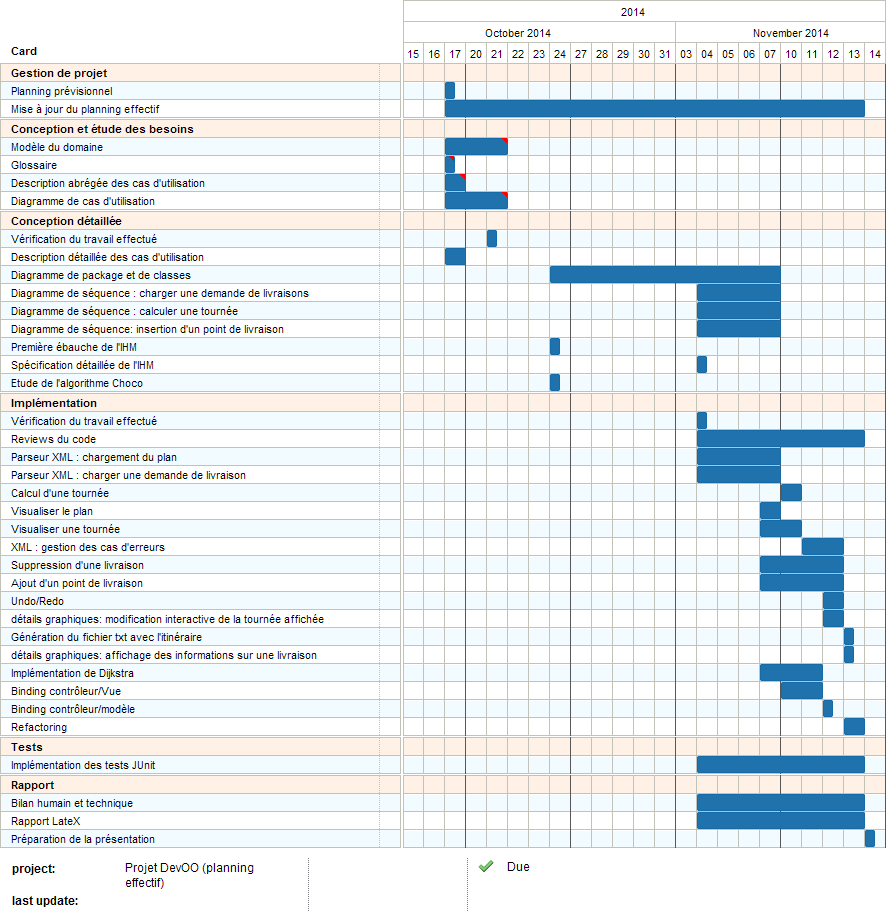
\includegraphics[width=\textwidth,height=\textheight,keepaspectratio]{Figures/effective_plan}
		\rule{35em}{0.5pt}
	\caption[Planning effectif du projet]{Planning effectif du projet}
\end{figure}
\clearpage

%----------------------------------------------------------------------------------------
%	SECTION 2
%----------------------------------------------------------------------------------------

\section{Bilan humain}

Ce projet est parfaitement adapté à l'exercice des méthodologies apprises en cours. Il nous a en effet permis de d'effectuer une gestion de projet importante, en particulier l'évaluation des durées des tâches, la répartition des rôles, la gestion du planning pour respecter les échéances critiques.
Nous avons également eu l'opportunité de réaliser un système en collaboration avec des clients, ce qui nous a permis de comprendre l'importance du dialogue continu avec le client, et l'importance de ses besoins et exigences dans la conception et la réalisation de l'application. 

Nous avons adopté le processus de développement agile \textbf{Gitflow} pour gérer le travail en groupe.Ce processus permet de travailler dans une branche sur une fonctionnalité indépendante qu'on intègre à la branche de production principale une fois qu'elle est complète. Cela permet de faciliter l'intégration continue et de minimiser les conflits.

Nous avons également mis en place une démarche de \textbf{code reviews}, où ne peut intégrer une nouvelle fonctionnalité qu'une fois que le code ait été revu et validé par un autre membre du groupe. Cela a permis à tous les membres du groupe de contrôler en continu la qualité du du code et de rester au fait de l'avancée du projet, notamment des parties qu'ils n'ont pas implémentées.

Nous avons néanmoins passé beaucoup de temps sur la partie modélisation et conception de notre application, en particulier sur la réalisation des diagrammes de séquences, et nous n'avons donc pu commencer l'implémentation que lors de la dernière séance du projet. Nous attribuons ce retard au fait que nous n'avons pas consacré du temps hors-séances à ce projet. Cependant, notre conception était solide, ce qui nous a permis d'avancer rapidement lors de l'implémentation.  

\section{Bilan technique}

Durant toute la progression du projet, nous avons appris à concevoir une application et appréhender l’importance de cette étape. En effet, les différents diagrammes rélisés nous ont permis de clarifier le développement et d’éviter les dérives. Nous avons remarqué lors de l’implémentation qu’une bonne conception permet de passer outre nombre de conflits et de faciliter l’intégration continue.

Concernant la programmation Java et SWING, notre formation premier cycle nous avait déjà fourni les clés pour créer une interface graphique dans ce langage. 

Pour conclure, la plus-value est plus méthodologique que technique.
